\subsection{Introduction and plan of this chapter}

In this chapter we will present three NP-completeness results. First
one, hardness of fp+r+cv we will present as reduction from Set Cover
variant, where every set has cardinality exactly 3. Second one,
hardness of ma+r+fp we will present as reduction from Three
Dimensional Perfect Matching. Hardness of those problems result in
hardness of extended models: we can add bandwidth and multiple
assignment to fp+r+cv; we can add bandwidth and communication to
ma+r+fp.

It seems that replication is the property of models which makes them
hard. Therefore we decided to investigate how much we can constrain
replication and still have NP-hard problems. As last section of this
chapter we will investigate restricting replication to have at most 2
replicas of each chunk type. It turns out that this variant remains
NP-complete, when it is paired with bandwidth. Our technique is to use
$3SAT$ as a problem which we reduce from.

\subsection{NP-hardness of model without bandwidth}

Set cover problem is well-known NP-complete problem. Other names that
we can find this problem in literature is Hitting set problem. Many variants of
this problem remain NP-complete. One of those variants is Set cover
with restriction that every set has cardinality exactly three. We will
use this $3SC$ problem as the problem we will reduce from.

Comment:There they say that 3HS in NP-complete:
\url{http://lcbb4.epfl.ch/reading/hitting\%20set/2003-niedermeierFPT3HS.pdf}
\url{http://www.sciencedirect.com/science/article/pii/S1570866703000091}

We will exploit the fact that we can construct $\VCNB$ instance where
we set number of VMs to spawn to be greater than number of chunk
types. Those excessive VMs are not processing any chunks but they are
still communicating with eachother as well as with processing
VMs.

First, we need to take decision variant of $3SC$. It is stated the
following way. We are given the universe $U$, family of universe
subsets $S = \{ S_1, S_2, \ldots, S_n \}$ with cardinality of each set
being three, and integer $k$. The problem is to decide whether there
exist a subfamily of sets $S' \subset S$ of cardinality $k$ that
covers every element in universe.

\subsubsection{Construction}

Idea of the construction is to create a chunk type for every element
of universe, and encode each subset $S_i$ as a gadget that contains
replicas of chunks that correspond to its elements. Here it is crucial
to use replication, as sets share elements of universe. Set $S_i$ is
chosen in $3SC$ instance when it has $3$ VMs spawned in it. Processing
each chunk will correspond to covering all the elements.


Let's take an instance $I$ of $3SC$. We will create VC instance $\VCNB_I$ in following
way. Let's start by setting integer constants in our instance:
\begin{itemize}
\item set transportation cost to some huge constant $\CostTrans = W$
  with idea of forbidding transportation. We will show how to
  calculate $W$ in an appendix, right now we can think about it as $W
  = \infty$.
\item set communication cost to $\CostCom = 1$
\item set number of VMS to $\Vms = 3 \cdot k$
\item set $\Thr =  3 \cdot k + 3 \cdot 3 \cdot 2 \cdot (k - 1)$
\end{itemize}


Then we construct the tree $\Tree_I$. It will have height 2 counted in number of
edges. It will consist of gadgets for every set $S_i$. Every gadget
consists of inner node and three leaves. We place three chunks in
every gadget; those chunks correspond to elements of $S_i$.

\subsubsection{Proof of correctness}

Crucial property of communication cost is that VMs should stick
closely to eachother to incline minimal cost. Therefore, before
prooving correctness of our reduction we need following lemma:

\begin{lemma}
In every $\VCNB$ solution $\Sol$ of cost $\leq \Thr$ we have exactly
$3$ VMs in $k$ gadgets and rest of the $n-k$ gadgets remain empty.
\end{lemma}
\begin{proof}
First, we notice that it is never beneficial to
transport chunks, as $W$ is already exceeding $\Thr$. Also we know that
$\Sol$ is feasible, therefore $|U|$ VMs sit on top of the chunks they
are processing.

Let's look at every pair of VMs that communicate. We
will count how many VMs communicate over 2 hop and how many
communicate over 4 hops. We do it by starting with 4 hops
communication and subtracting 2 hops for every pair of VMs that sit in
the same gadget. We notice that with constant number of VMs to spawn,
the more gadgets containing VMs the less 2 hop communications there
are. Communication cost is optimal when every gadget contains exactly
3 VMs, because then we subtract 3 pair. We chosen $\Thr$ to be exactly
the cost of such solution. Therefore, no solution that spawns VMs in
more than $k$ gadgets will ever have cost $\leq \Thr$.
\end{proof}

\begin{theorem}
$I \in 3SC$ iff $\VCNB_I$ has solution of cost $\leq \Thr$.
\end{theorem}
\begin{proof}

($=>$) Let's take the covering set $S = \{S_1, S_2, \ldots, S_k\}$ and place $3$ VMs in each gadget that
corresponds to every set of $S$. We match VMs to chunks the following
way: we traverse VMs one by one, and if the VM sit on top of the chunk
type that was not yet processed, we match that them; otherwise we set
the VM to be idle. Let's calculate the cost of the solution:
\begin{itemize}
\item communication cost inside gadget is $2 \cdot {3 \choose 2}$,
  because we take every pair and add 2 hop communication cost
\item communication cost from single gadget to all other gadgets is $4
  \cdot 3 \cdot 3 \cdot (k - 1) / 2$, where $2$ is a factor inclined by
  communication over $4$ hops, $3$ is the number of VMs in the gadget,
  $3 \cdot (k-1)$ is the number of VMs that sit in other gadgets, and
  $/2$ is inclined by counting every pair twice
\end{itemize}

By summing above costs over every of $k$ gadgets, we have cost equal
to $\Thr$.

($<=$) Let's take VC solution. First, we apply our lemma that in $\leq
\Thr$-cost
solution $k$ gadgets are full of VMs. We construct our hitting set from
sets that correspond to those full gadgets. Also, we know that every
chunk type was processed. Therefore every element of universe was hit.
\end{proof}

\subsection{NP-completeness of MA+FP+R}

3D exact matching introduction here.

\subsubsection{Construction}

\begin{itemize}
\item tree consists of gadgets for each triple
\item chunks correspond to elements of X,Y and Z
\item $|X| = |Y| = |Z| = k$
\item we set TC to 1
\item we set m to 3
\item we set number of VMs to $k$
\item we set threshold to $2 \cdot 2 \cdot k$
\item each gadget consists of 3 leaves and parent; in leaves there are
  chunks that correspond to elements of a triple
\end{itemize}

\subsubsection{Proof}

($=>$) Let's take solution to 3D exact matching. We spawn VM in every
gadget that corresponds to chosen triples. We match every chunk in a
gadget to machine in this gadget (only for chosen ones). Solution has
cost exactly $\Thr$.

($<=$) Let's take solution to $VC$ instance of cost $\leq \Thr$. We
chose triples that correspond to gadgets where were VMs. Everything
was processed, therefore every element of X,Y and Z is matched.
\subsection{NP-completeness of model with bandwidth -
 3SAT introduction}

We decided to make reduction from Boolean Satisfiability problem (SAT)
to our Virtual Cluster problem with bandwidth (VCB). SAT is decision
problem, but VCB is optimization problem with NO answer
possible. Therefore to make those problems compatible in terms of
reduction, we consider decision VCB variant, in which instance we have
additional constant $\Thr$, and instance belongs to VCB if it has feasible
solution of cost $\leq \Thr$.

Let's remind what decision VCB variant instance consists of:
\begin{enumerate}
\item balanced rooted tree $\Tree$
\item edge capacities $\Bandwidth(e)$
\item constants $\CostTrans$, $\CostCom$, which are costs of chunk transfer and
communication
\item constant $\Vms$, which is desired number of VMs to be spawned
\item constant $\ChunkTypes$, which is number of types of chunks
\item sequence of chunks placed in leaves of $\Tree$, possibly replicated
\item constant $\Thr$
\end{enumerate}

Let's remind what $\SAT$ instance consists of:
\begin{enumerate}
\item clauses (let's name number of clauses as $\Clauses$)
\item literals
\item variables (let's name number of variables as $\Vars$
\end{enumerate}

\subsubsection{Construction}
Let's take any formula in Conjunctive Normal Form, name it $\Formula$ and produce
VCB instance $\VCB_{\Formula}$. First, construct the tree $\Tree_{\Formula}$. It will consist of
a root and separate gadget for each variable of $\Formula$, each of which
is a child of the root.


Gadget for variable $x$ has its root, $var(x)$, and two children:
$\positive(x)$ and $\negative(x)$. Vertex $\positive(x)$ has $\NClauses$
children: $x_1, x_2, \ldots, x_{\NClauses}$. Vertex $\negative(x)$ has
$\NClauses$ children: $\neg x_1, \neg x_2, \dots, x_{\NClauses}$. Every
gadget has the same structure: the same height, the same number of
leaves, and the same height. In fact, we will set bandwidth to be the
same everywhere in every gadget. Differences will be shown when we
will place data chunks.

We set number of virtual machines to $v = \NClauses \cdot \NVars$.

Now we will set cost of chunk transportation and cost of communication
among virtual machines. We set communication cost to be $1$. We set
trasportation cost to be $\CostTrans = W$, where $W$ is constant large enough
to disallow transportation. It means that if virtual machine wants to
process the chunk, it has to be spawned where the data chunk is
placed. Technically, transportation is not completely disallowed, it
just inclines cost so huge that every optimal solution has no
trasportation. TODO: We show how to compute $W$ in appendix.

Now we will set bandwidth constraints in $\Tree_{\Formula}$. There are three
levels of edges in $\Tree_{\Formula}$: top, middle and bottom. We set
bandwidth to unlimited at levels bottom and middle. At every edge of
top level, we set the same bandwidth to: $\NClauses \cdot (\NVars -
\NClauses)$.

We set number of chunk types to be equal to number of clauses, $\ChunkTypes =
\NClauses$. To finish construction of $\Tree_{\Formula}$, we need to place data chunks in
leaves. We do it the following way. For each clause of number $i$ we
construct as many replicas of chunk $c_i$ as there are literals in
clause $i$. For each literal $l$ (of form $x$ or $\neg x$) that satisfies clause $i$ we place
replica of chunk $c_i$ in leaf labeled $c_{l_i}$.

To finish our construction, we need to set value of constant $\Thr$.

 We
do it by calculating communication cost among spawned virtual machines in
certain solution to our instance. This soulution is constructed by placing
virtual machines in all leaves of $positive(v)$ and none in leaves
$negative(v)$ for every gadget for variable $v$. Please note that $Th$
computed such way do not contain transportation cost. TODO: calculate
$Th$ in appendix.

\subsubsection{Proof of correctness of construction}

With our construction completed, we need to prove that it indeed
decides SAT.

Idea behind capacity of set amount is that in every gadget we can
spawn at most $cl(\Psi)$ virtual machines. Let's prove it formally:

\begin{lemma} (bandwidth lemma)
  Let $c$ and $v > 4$ be positive natural numbers. Let $a_1, a_2, \ldots,
  a_v$ be natural number sequence that adds up to $c \cdot v$. Also, for
  each $i$ we have $a_i \leq 2 \cdot c$. Then, if we have this:

  $$ \forall_i a_i \cdot (c \cdot v - a_i) \leq c \cdot (c \cdot v -
  c) $$

  then each $a_i = c$.
\end{lemma}
\begin{proof}

Let's assume the contrary, which means that there exists such $y$ that
$a_y \neq c$. Then there are two cases: first, $a_y>c$ and second,
$a_y<c$. Proof for the first case is presented below; second case
with pidgeon hole principle results in existance of $a_z > c$, which
is basically the same (just substitute $a_y := a_z$ in proof below).

As we have $a_y < 2c$, we can say that $a_y$ has form $c +
k$ for $k \in [1, \ldots, c]$. Let's look at bandwidth inequality:

$$ (c + k) \cdot (c \cdot v - c - k) \leq c \cdot (c \cdot v - c) $$

After transforming it we have:

$$ 0 \leq k(k - (c \cdot (v - 2))) $$

Which is true for $k \leq 0$ or $k \geq c \cdot (v - 2)$, so no
positive $k \leq c$ can satisfy this inequality for $v > 4$, which gives a contradiction.

\qed

\end{proof}

We will apply this lemma in following way. We interpret $a_i$ as
number of VMs that are spawned in $i$-th gadget. We set $c$ as number
of clauses and $v$ as number of variables. LHS of inequality from the
lemma is formula for communication cost of machines inside $i$-th
gadget to machines outside the gadget. RHS of the inequality is
bandwidth constraint for the gadget. Corollary from the lemma is that
any feasible solution must place exactly $c$ machines in every gadget.

TODO: We need to consider case where $v \leq 4$. We can say that we
restrict formulas to have 4 or more variables. This subset of $SAT$ remains NP-complete.

\begin{theorem}Formula $\Psi$ is satisfiable iff $VCB_{\Psi}$ has
solution of cost $\leq Th$.
\end{theorem}

\begin{proof}
($=>$) Let's take any valuation $F$ that satisfies $\Psi$. We will construct
solution to $VCB_{\Psi}$ using F in the following way. For each
variable $v \in var(\Psi)$ we place $cl(\Psi)$ virtual machines in
leaves of gadget $var(v)$. We need to choose $cl(\Psi)$ out of
$2 \cdot cl(\Psi)$ leaves to spawn VMs. If $F(v) = 1$, we spawn all VMs in leaves
of $positive(v)$, else we spawn all VMs in leaves of
$negative(v)$. Solution constructed such way has cost exactly
$Th$, because VMs are evenly splitted among gadgets and VMs are not
mixed between $positive(v)$ and $negative(v)$ subtrees.

We calculate the matching of chunks to VMs by matching every chunk to
VM that sits on top of first chunk replica. This solution is feasible
(every chunk type is processed) basically
because given valuation satisfied the $\Phi$.

Now we will show that this solution has indeed cost exactly $Th$. We have to
take only communication cost. This holds because of the bandwidth lemma.

($<=$) Let's take any solution to $VCB_{\Psi}$ of cost $\leq Th$. We
will construct valuation $F$ using placement of virtual machines in
solution to $VCB_{\Psi}$.

We need to take following observations. In every solution of cost
$\leq Th$ every gadget has exactly $ch(\Psi)$ VMs spawned in its
leaves. It is true because we proved the bandwidth lemma. Also, inside
every gadget either all VMs are spawned in $positive(v)$ or all VMs
are spawned in $negative(v)$. It is true because cost of solution
where at least one gadget has VMs mixed between those branches is
always greater than $Th$.

TODO: prove it more formally. First, define semi-feasible solution. Let's take any $p,q$ being number of VMs
spawned in left and right subtree. Then we say that we can improve the
solution by moving all $q$ to where $p$s lie and we have cheaper solution.

Now we can construct our valuation $F$. We do it the following way
(for each $v \in var(\Psi)$:

\begin{itemize}
\item if $v_1$ has machine in it then $F(v) = true$
\item otherwise $F(v) = false$
\end{itemize}

Valuation $F$ satisfies $\Psi$ because it satisfies every clauses, as
$VCB_{\Psi}$ solution processed all the chunks. To see it, let's take
any clause chunk and see in which leaf it was processed. We take a
look at label of this leaf. The label is a literal that is a whiteness
to truthness of this clause.
\end{proof}

\subsection{NP-completeness of model with bandwidth and replication of
  degree 2.
}


The idea is to reduce from 3SAT using only replication of degree
$2$. How can we simulate this behavior using only two replicas? First,
let's reduce from $3SAT$ instead of $SAT$. Our tree $T_{\Psi}$
will consist of two types of gadgets: gadgets for variables and
gadgets for clauses. Most fundamental conceptual difference is that
for every clause we create three chunk types instead of just one (like
in previous proof).

\subsubsection{Construction.}

We put chunks in following way. First, we put clause chunks in
variable gadgets like we did in proof of NP-completeness of 3 replica
model with the difference that now we place distinct chunks instead of
three copies of the same chunk.  Secondly, we place three chunks that
correspond to clause in all three leaves of their clausule gadgets. We
place in total $6 \cdot c$ variable chunks chunks this way.

We set number of spawned VMs to $cv + 2c$. Our intention is that in
every variable gadget there will lie $c$ VMs and in every of clause
gadgets there will lie $2$ VMs.

We set bandwidth for top edge of each variable gadget to:

$$ bw(v) = 3  \cdot  3  \cdot  (3  \cdot  (v - 1) + 2  \cdot  c) $$


First factor is distance on tree which is 6 divided by 2 (which is a
factor caused by counting every communication twice). Second factor is
number of VMs that spawn in every variable gadget. First compound of a
sum is 3 times number of outer variable gadgets. Second compound of a
sum is number of VMs that spawn in each of c clause gadgets.

We set bandwidth for top edge of each clause gadget to:

$$ bw(c) = 3  \cdot  2  \cdot  (2  \cdot  (c - 1) + 3  \cdot  v) $$

\subsubsection{Proof of correctness of the construction.}

\begin{lemma}
Exactly $c$ VMs are forced to spawn in every of $v$ variable gadgets
and exactly $2$ VMs are forced to spawn in every of $c$ clause gadgets
in every solution of cost $\leq Th$.
\end{lemma}

\begin{proof}
We show it by using bandwidth constraints. We have to take into
consideration following communication paths: (1) communication to
other variable gadgets; (2) communication to clause gadgets Extended
bandwidth lemma. In every solution of cost $\leq Th$ we have exactly
$c$ VMs in each variable gadget and $2$ VMs in each clause gadget.

\end{proof}

\begin{theorem}Constructed $VCB$ instance has solution of cost $\leq
  Th \iff \Formula \in 3SAT$.
\end{theorem}

\begin{proof}
($=>$) If we have a valuation, we fill variable gadgets with VMs like in
proofs before. Then we fill $2 \cdot c$ VMs in following way:

\begin{itemize}
\item if first literal satisfied the clause, we put $2$ VMs in second and
third leaf of clause gadget
\item if first literal not satisified the clause, we put $2$ VMs in first
and second leaf of clause gadget
\end{itemize}

We compute matching of chunks to VMs in the following way:
\begin{itemize}
\item chunk $c_i^1$ is matched to VM that sits in variable gadget; there
should be one like that, because the valuation satisfies
\item chunks $c_i^2$ and $c_i^3$ are matched to VMs that sit in clause
gadgets; there exists minimal-cost solution where VMs sit there
\end{itemize}

We produced feasible solution of cost $\Thr$, because there were no
transport and VMs communicated in predicted way.

($<=$) In order to finish the proof, we must prove the existance of
valuation that satisfies $\Formula$.
Let's take any solution $\Sol$ to $\VCNB_{\Formula}$ instance of cost $\leq \Thr$.

We create valuation Val in following way:
\begin{itemize}
\item $\Val(v) = T$ iff there lies VM on first leaf on positive side of $v$ gadget in $SOL$
\item $\Val(v) = F$ otherwise
\end{itemize}

\begin{lemma}For every clause there exist a VM in variable gadget that processes one of
  3 chunks that correspond to that clause.
\end{lemma}
\begin{proof}
 Every of $3$ chunks that correspond to every clause has machine sitting
on top of it. At least one of those $3$ is not idle in a variable gadget
- otherwise those two VMs in clause gadgets would not suffice in
satisfying all chunk types.\end{proof}

Observation. It might happen that in $SOL$ $2$ VMs in
clause variables are idle, and $3$ VMs in variable gadgets are
processing those $3$ chunk types, then we can take arbitrary in the rest
of the proof.


\begin{lemma}$\Val$ satisfies $\Formula$.
\end{lemma}
\begin{proof}
Let's take matching $M$ of $\Sol$. Let's take arbitrary clause of
$\Formula$ and its $3$ chunk types
: $c_i^1, c_i^2, c_i^3$. Let's name machines corresponding to them
to $vm_i^1, vm_i^2, vm_i^3$. Two of those lie in clause gadgets. Let's
take the chunk type that was processed in variable
gadgets and look at where it was processed. Look how was labeled the
leaf the VM lies. In our valuation Val we set this literal to have
value True. Therefore the clause is satisfied.
\end{proof}

This last lemma proves our theorem.
\end{proof}
\subsection{Images}

\begin{figure}[htbp]
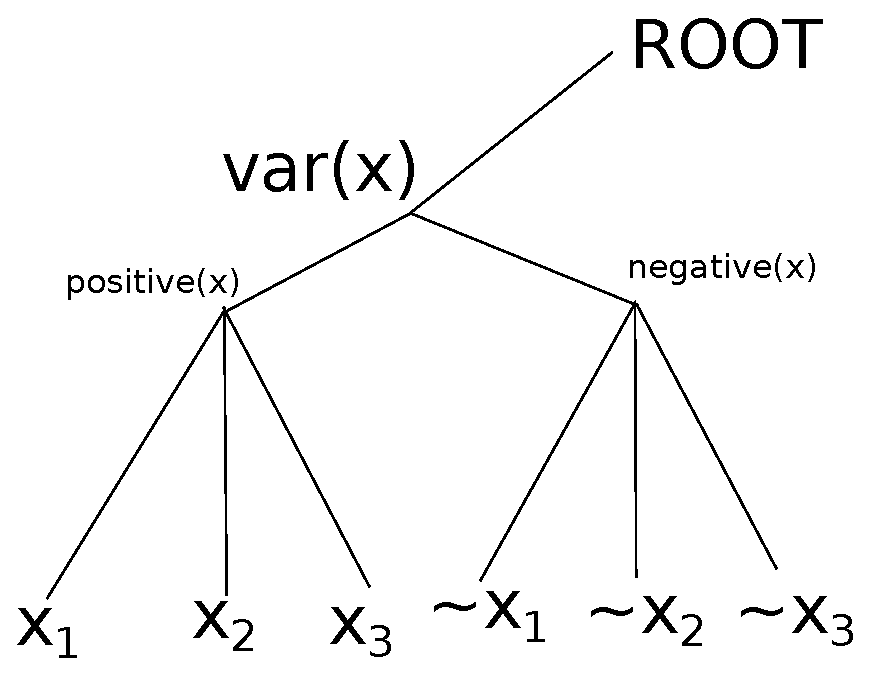
\includegraphics[width = \columnwidth]{figs/gadget-no-bw}
\end{figure}


\begin{figure}[htbp]
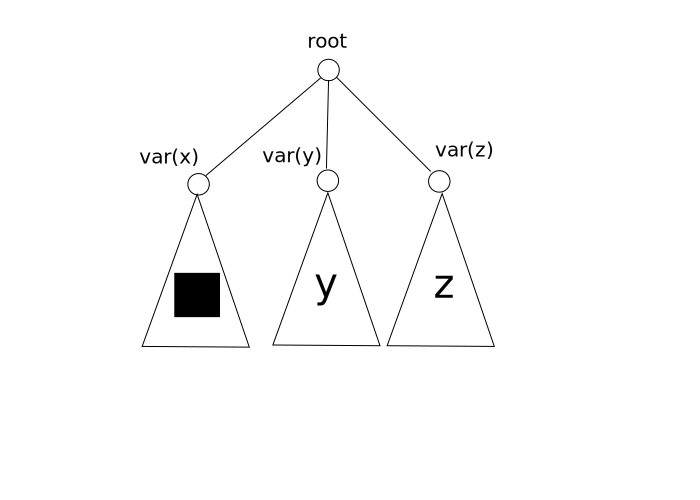
\includegraphics[width = \columnwidth]{figs/vc-instance}
\end{figure}


\begin{figure}[htbp]
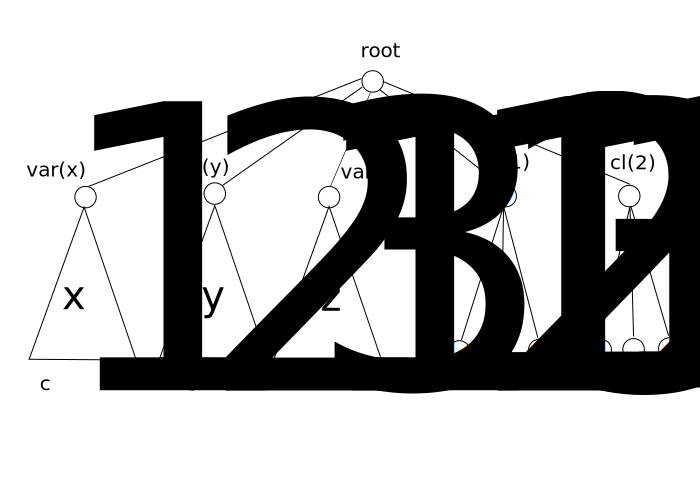
\includegraphics[width = \columnwidth]{figs/vc-instance-r2}
\end{figure}


\begin{figure}[htbp]
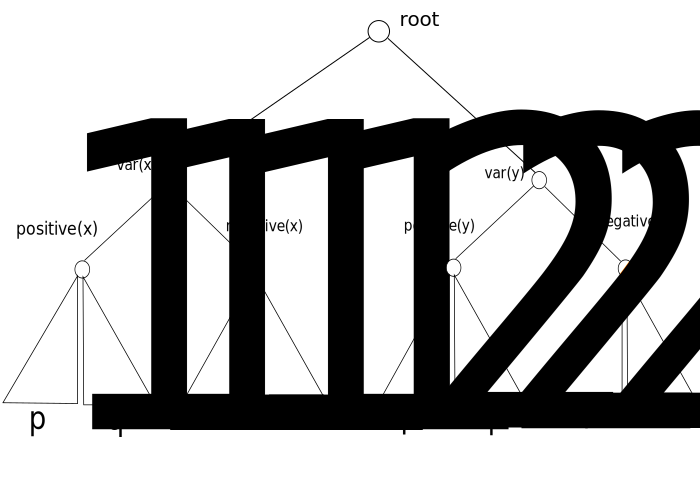
\includegraphics[width = \columnwidth]{figs/lemma-two-gadgets}
\end{figure}


\begin{figure}[htbp]
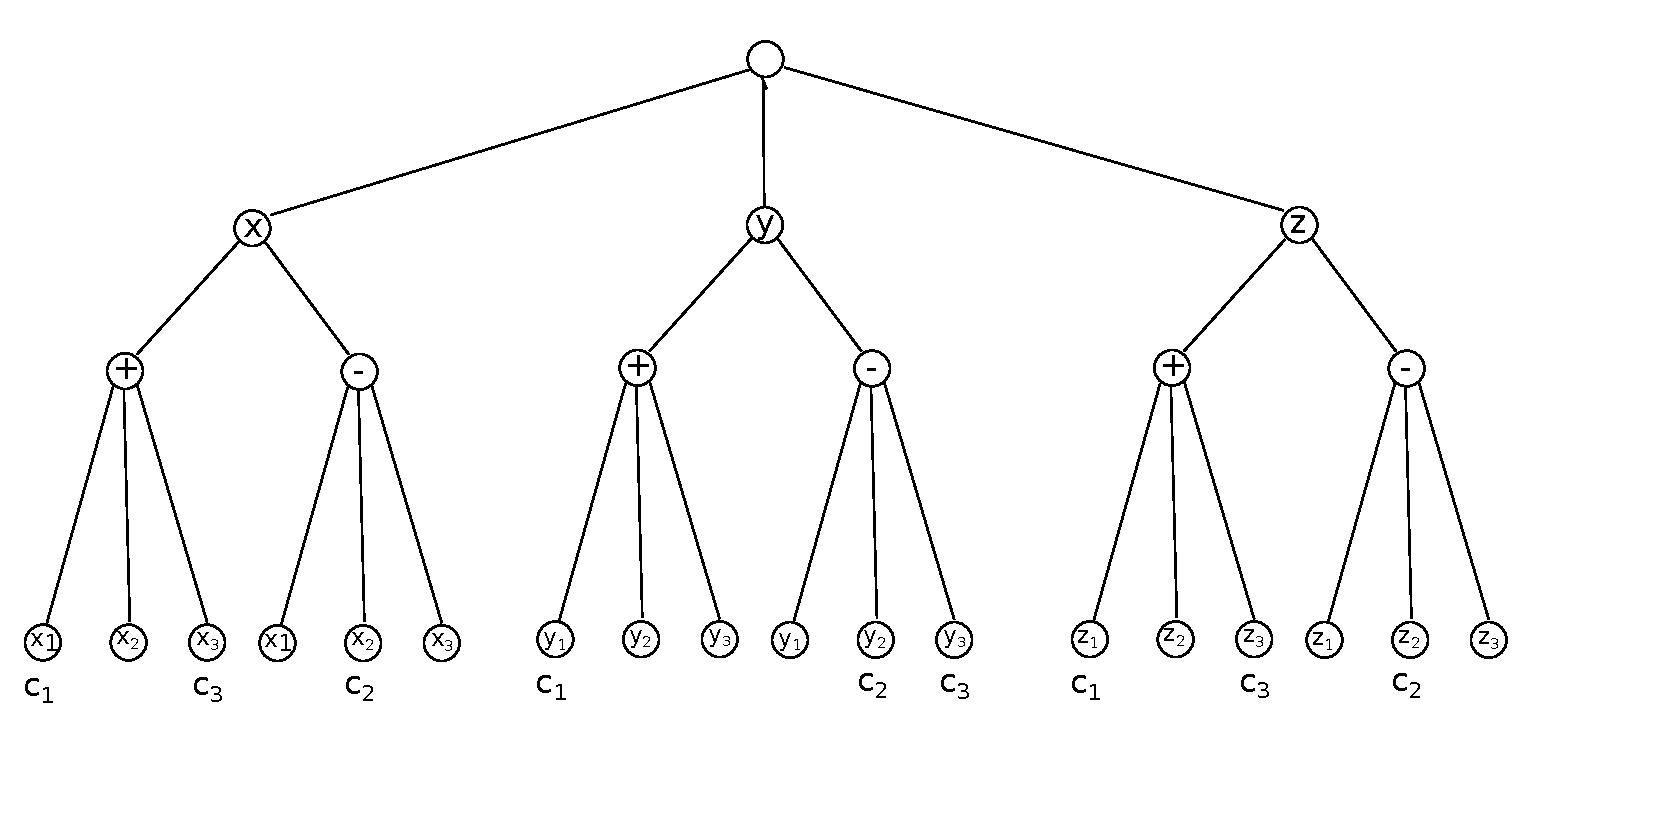
\includegraphics[width = \columnwidth]{figs/formula-example}
\end{figure}

